
%(BEGIN_QUESTION)
% Copyright 2010, Tony R. Kuphaldt, released under the Creative Commons Attribution License (v 1.0)
% This means you may do almost anything with this work of mine, so long as you give me proper credit

Suppose we have an Allen-Bradley MicroLogix 1000 PLC connected to two liquid level switches installed in the same tank, controlling a solenoid valve to empty liquid out of that tank:

$$\includegraphics[width=15.5cm]{i02257x01.eps}$$

We wish for the solenoid valve to energize and open when the liquid level in the tank reaches 4.5 feet, then de-energize and shut when the liquid level falls to 3 feet.  Write a RLL program for the PLC (complete with correct address labels for each of the virtual contacts) to fulfill this function:

$$
\includegraphics[width=15.5cm]{i02257x02.eps}$$

\vfil

\underbar{file i02257}
\eject
%(END_QUESTION)





%(BEGIN_ANSWER)

This is a graded question -- no answers or hints given!

%(END_ANSWER)





%(BEGIN_NOTES)

When we read the requirements of this system -- to energize the solenoid at the high-level point and de-energize it at the low-level point, we know we need {\it hysteretic} behavior: what we need is for the solenoid to be turned on and off with a 1.5 foot ``deadband'' action.  Only a latching PLC program will be able to accomplish this feat.

The program we need this PLC to execute is not unlike a motor start/stop control, where one input causes the motor to start and the other causes it to stop, with the PLC ``latching'' the motor's state in between switching events.  Thus, we may develop a solution using retentive coil instructions, or by using the more traditional ``seal-in'' feedback algorithm whereby a standard coil instruction controls the motor's state, and a contact instruction addressed to that same bit keeps the motor in its last state.

\vskip 10pt

Solution using retentive coil instructions (``latch'' and ``unlatch''):

$$\includegraphics[width=15.5cm]{i02257x03.eps}$$

\vskip 10pt

Solution using a standard coil instruction with a seal-in contact:

$$\includegraphics[width=15.5cm]{i02257x04.eps}$$

%INDEX% PLC, ladder logic programming: sketching a solution to a problem

%(END_NOTES)


